\documentclass[12pt]{article} 
\usepackage[utf8]{inputenc}
\usepackage{geometry}
\geometry{letterpaper}
\usepackage{graphicx} 
\usepackage{parskip}
\usepackage{booktabs}
\usepackage{array} 
\usepackage{paralist} 
\usepackage{verbatim}
\usepackage{subfig}
\usepackage{fancyhdr}
\usepackage{sectsty}

\pagestyle{fancy}
\renewcommand{\headrulewidth}{0pt} 
\lhead{}\chead{}\rhead{}
\lfoot{}\cfoot{\thepage}\rfoot{}


%%% ToC (table of contents) APPEARANCE
\usepackage[nottoc,notlof,notlot]{tocbibind} 
\usepackage[titles,subfigure]{tocloft}
\renewcommand{\cftsecfont}{\rmfamily\mdseries\upshape}
\renewcommand{\cftsecpagefont}{\rmfamily\mdseries\upshape} %

\usepackage{amsmath}
\usepackage{amssymb}
\usepackage{empheq}
\usepackage{xcolor}
\usepackage{bbm}
\renewcommand{\L}[1]{\mathcal{L}\{#1\}}
\newcommand{\ans}[1]{\boxed{\text{#1}}}
\newcommand{\vecs}[1]{\langle #1\rangle}
\renewcommand{\hat}[1]{\widehat{#1}}
\newcommand{\F}[1]{\mathcal{F}(#1)}
\renewcommand{\P}{\mathbb{P}}
\newcommand{\R}{\mathbb{R}}
\newcommand{\qed}{\quad \blacksquare}
\newcommand{\brak}[1]{\left\langle #1 \right\rangle}
\newcommand{\C}{\mathbb{C}}
\newcommand{\bra}[1]{\left\langle #1 \right\vert }
\newcommand{\ket}[1]{\left\vert #1 \right\rangle}
\newcommand{\E}{\mathbb{E}}
\newcommand{\ind}{\mathbbm{1}}

\usepackage{tikz}
\usepackage{pgfplots}
\pgfplotsset{compat=1.18}

\title{APMA 1930W: Probabilities in Quantum Mechanics}
\author{Milan Capoor}
\date{Fall 2023}

\begin{document}
\maketitle
\section*{Lecture 1: Sept 6}
Outline of the course:
\begin{enumerate}
    \item A single particle
    \begin{itemize}
        \item Probabilities
        \item Waves
    \end{itemize}

    \item Entanglement (multiple particles)
    \item Applications and consequences
    \begin{itemize}
        \item Bell's theorem
        \item Teleportation
        \item Free will (Conway-Kochen theorem)
        \item Encryption
        \item Quantum computing 
    \end{itemize}
\end{enumerate}

\section*{Lecture 2: Sept 8}
\subsection*{The 2-Slit Experiment}
\textbf{A wave:} we can imagine a 1-color wave at a single frequency
\[A\cos(\omega t - kx + \phi)\]
where 
\begin{itemize}
    \item $\omega$ is the frequency (rad/s) which describes the speed of vertical oscillation
    \item $k$ is rad/m which describes speed of horizontal movement
    \item $\phi$ is the phase shift 
    \item $A$ is the amplitude 
\end{itemize}

(the goal of the $kx$ term is to grow proportionally with the $\omega t$ term to create a constant value without oscillation to send through the detector)

This wave can be decomposed:
\[A\cos(\omega t - kx + \phi) = A\cos \phi \cos(\omega t - kx) - A\sin \phi \sin(\omega t - kx)\]

\emph{Proof:}

Using Euler's identity, $e^{iz} = \cos z + i\sin z$, 
\begin{align*}
    \Re(A \cos(\omega t - kx + \phi)) &= \Re(A e^{i(\omega t - kx + \phi)})\\
    &= \Re(Ae^{i \phi} (\cos(\omega t - kx) + i\sin (\omega t - kx)))\\
    &= \Re(A(\cos \phi + i \sin \phi) (\cos(\omega t - kx) + i\sin (\omega t - kx)))\\
    &=  A\cos \phi \cos(\omega t - kx) - A\sin \phi \sin(\omega t - kx)
\end{align*}

\textbf{The Experiment:}
We imagine a variable with two narrow slits bombarded by the wave $\tilde A \cos(\omega t - kx)$.

Our goal is to find the equation of the wave impacting a detector at $x=1$ after the diffusion effect of the variable. Because there are two slits, the waves ($\psi_1, \psi_2$) from each slit will interfere (linear sum) to create a new wave on the detector at a specific point $\psi(x, y, t)$ after traveling a distance $r_1$ or $r_2$ respectively. Thus,
\[\psi(x, y, t) = \psi_1(x, y, t) + \psi(x, y, t) = A_1 \cos(\omega t - k r_1) + A_2(\cos(\omega t - k r_2))\]
where $A_1 = \tilde A/\sqrt{r_1}$ and $A_2 = \tilde A/\sqrt{r_2}$ to take into account fading intensity over time.

All of this together will give us the amplitude of composite waves at the point on the screen which we square to get the intensity ($I \propto A^2$)

Calculated across the entire screen this will give a distribution of intensities which \textbf{perfectly} matches the distribution of collision locations of single-particles over a long period of time. 

\section*{Lecture 3: Sept 11}
\subsection*{Stern-Gerlach Experiment}
We set up two non-symmetric magnets on top of each other with North pole facing South pole and a gap between them. We send an electron through and it will either go up or down to land on two specific points on the detector, indicating that each electron has a magnetic moment of exactly $\hbar/2$ or $-\hbar/2$.

Important findings:
\begin{enumerate}
    \item This happens for ANY orientation of the machine
    \item The result is definite. If we put a second S-G device at the detector point, ALL the particles that went up the first time will also go up the second time (and the same for down). That is,
    
    \[\P(\lambda_n(t + 1) = 1 | \lambda_n(t) = 1) = 1, \quad \P(\lambda_n(t + 1)=  1 | \lambda_n(t) = -1) = 0\]
    where $\lambda_n$ is the state of the particle after going through the device ($\lambda_n : t \mapsto \{-1, 1\}$)
\end{enumerate}

If we now send the particle through a new ``m-machine'' characterized by a new orientation $n, m \in \R_1^3 = \{v \in \R^3 : |v| = 1\} = S^2$, then the corresponding probabilities for a particle prepared in the $n$-direction is 
\begin{align*}
    \P(\lambda_m(t + 1) = 1 | \lambda_n(t) = 1) = \frac{1 + m \cdot n}{2}\\
    \P(\lambda_m(t + 1) = 1 | \lambda_n(t) = 1) = \frac{1 - m \cdot n}{2}
\end{align*}

Now we create a new experiment. A stream of N $\lambda_x = 1$ particles go through an orthogonal $z$-detector such that $\P(\lambda_z = 1) = N/2$ and $\P(\lambda_z = -1) = N/2$. If we magnetically bend these two back through the same $x$-detector so the input is 1/2 $\lambda_z = 1$ and 1/2 $\lambda_z = -1$, we still see $\P(\lambda_x = 1) = N$. 

But! If we do not bend these into the same detector but place another $x$-detector after the $z$-detector we find that $\P(\lambda_x = 1 | \lambda_z = 1) = N/4$ and $\P(\lambda_x = -1 | \lambda_z = -1 ) = N/4$ -- exactly what would have happened regardless of the earlier $x$-detector

\section*{Lecture 4: Sept 13}
\textbf{Feynman's Version:}
Using three machines in series, we are able to take an input, split it, and put it back together regardless of preparation. Using the normal process, we prepare $\lambda_x = 1$ then send it through one $z$-Feynman machine with the bottom blocked (so $\P(\lambda_z = 1) = N/2$) then through a $x$-Feynman machine with the top blocked so the final output is $\P(\lambda_x = -1) = N/4$

Now we set up a new experiment: send $\lambda_x = 1$ through a $z$-Feynman machine with no block then through a $x$-Feynman machine with the top blocked. The output is $0$.

\textbf{Conclusion:} bending the streams back together is as if we never sent it through a machine at all because the particle is now in both states. 

\subsection*{Derivation of State}
\textbf{Recall the Two-slit:} we use complex variables to account for phase and model linear interference (See Lecture 2)
\[\psi(y, t) = \Re(y)e^{i\psi(y, t)} = A_1(y) e^{-ikr_1(y)} + A_2(y)e^{-ikr_2(y)}\]

In the Two-Slit Experiment the outcomes fall into $\R^2$ but in teh Stern-Gerlach Experiment, there are only two possible outcomes. 

\section*{Lecture 5: Sept 15}
\subsection*{A Complex-valued Vector Space}
(The complex-values conveniently handle phase while the vector space accounts for linear interference)

Our first task is to determine the dimensionality needed. From the experiment itself, we saw that $\R_1^3$ was sufficient to completely determine the system. Thus we do not need a higher dimensional space than $\R^3$. In mapping to the complex numbers, though, we observe that $\mathbb{C}^2$ already provides more degrees of freedom than we need. 

\textbf{Notation:}

\begin{center}
    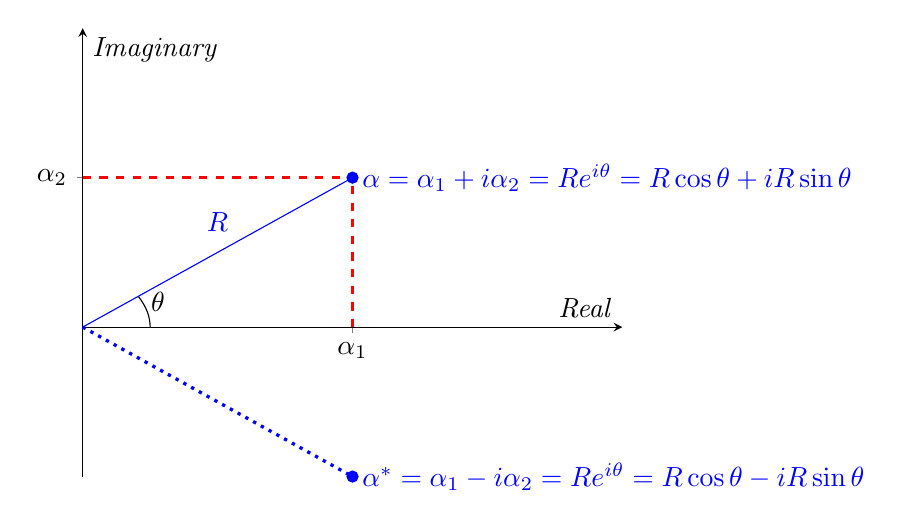
\begin{tikzpicture}
        \begin{axis}[
            axis lines=middle, 
            ylabel={\emph{Imaginary}}, 
            xlabel={\emph{Real}}, 
            xtick={1}, ytick={1},
            xticklabels={$\alpha_1$}, yticklabels={$\alpha_2$},
            xmax=2, ymax=2,
            clip=false]
            \addplot[dashed, red, very thick, domain=0:1]{1};
            \draw[dashed, red, very thick] (axis cs: 1, 0) -- (axis cs: 1, 1);
            \addplot[blue, domain=0:1]{x};
            \addplot[dotted, very thick, blue, domain=0:1]{-x};
            \draw (0.25, 0) arc (0:24:0.5) node[anchor=west, yshift=-2, xshift=1]{$\theta$};
            \filldraw[blue] (axis cs:1,1) circle (2pt) node[anchor=west]{$\alpha=\alpha_1 + i\alpha_2=Re^{i\theta} = R\cos\theta + iR\sin \theta$};
            \filldraw[blue] (axis cs:1,-1) circle (2pt) node[anchor=west]{$\alpha^*=\alpha_1 - i\alpha_2=Re^{i\theta} = R\cos\theta - iR\sin \theta$};
            \node[blue] at (axis cs: 0.5,0.7) {$R$};
        \end{axis}
    \end{tikzpicture}
\end{center}

This gives us several identities:
\[\R^2 = \alpha_1^2 + \alpha_2^2 = |\alpha|^2 = \alpha^* \alpha = (\alpha_1 - i\alpha_2)(\alpha_1 + i\alpha_2)\]

From these, we see for $a \in \mathbb{C}^2$ 
\begin{align*}
    a &= \begin{pmatrix}
        \alpha\\
        \beta
    \end{pmatrix} = \begin{pmatrix}
        \alpha_1 + i\alpha_2\\
        \beta_1 + i \beta_2
    \end{pmatrix}\\
    &\implies |a|^2 = |\alpha|^2 + |\beta|^2\\
    &= \alpha_1^2 + \alpha_2^2 + \beta_1^2 + \beta_2^2\\
    &= (\alpha^* \alpha) + (\beta^* \beta)\\
    &= \begin{pmatrix}
        \alpha_1 + i\alpha_2 & \beta_1 + i\beta_2
    \end{pmatrix}^* \begin{pmatrix}
        \alpha_1 + i\alpha_2\\
        \beta_1 + i\beta_2
    \end{pmatrix} \qquad (=a^\dagger a)\\
    &= \alpha_1^2 + \alpha_2^2 + \beta_1^2 + \beta_2^2\\
    &= \left|\begin{pmatrix}
        \alpha\\
        \beta
    \end{pmatrix}\right|^2
\end{align*}

($a^\dagger a$ is the composition of element-wise conjugate and transpose.)

\subsection*{Dirac Notation}
For $\psi \in \mathbb{C}^2$ we use $\bra{\psi}$ to designate the state of the particle corresponding to $\psi$. 

Then we define 
\[\ket{\psi} := \bra{\psi}^\dagger = \begin{pmatrix}
    \alpha\\
    \beta
\end{pmatrix}^{\dagger} = (\alpha^*, \beta^*)\]

So 
\[\brak{\psi | \psi} = \psi^\dagger \psi = |\psi|^2\]

\section*{Lecture 6: Sept 18}
\subsection*{A Better State Space}
Shortcomings of $\R_1^3$:
\begin{itemize}
    \item Nonlinear
    \item Arbitrary subset of a vector space
    \item No amplitudes
    \item Phase is difficult
\end{itemize}

\textbf{Complex Space:} $\mathbb{C} = \{\alpha_1 + i\alpha_2 | \alpha_1, \alpha_2 \in \R\}$ 

Which gives us a probability, 
\[|\alpha|^2 = \alpha_1^2 + \alpha_2^2 = \alpha^*\alpha\]

\textbf{2-Space:} $\mathbb{C}^2 = \{\begin{pmatrix}
    \alpha\\
    \beta
\end{pmatrix} : \alpha, \beta \in \C\}$

For which we introduce Dirac notation (Bra-Ket notation):
\[\ket{a} = \begin{pmatrix}
    \alpha\\\beta
\end{pmatrix}\]
so 
\[|\ket{a}|^2 = \brak{a | a} = \ket{a}^\dagger \ket{a} = \begin{pmatrix}
    \alpha^* & \beta^*
\end{pmatrix} \begin{pmatrix}
    \alpha\\
    \beta
\end{pmatrix} = |\alpha|^2 + |\beta|^2\]

\textbf{More generally:} 
\[\ket{a} = \begin{pmatrix}
    \alpha\\ \beta
\end{pmatrix}, \quad \ket{b} = \begin{pmatrix}
    \delta\\ \gamma
\end{pmatrix} \longrightarrow \brak{a | b} = \begin{pmatrix}
    \alpha\\ \beta
\end{pmatrix}^\dagger \begin{pmatrix}
    \delta\\ \gamma
\end{pmatrix} = \alpha^* \delta + \beta^* \gamma \]

We call $\brak{a | b}$ the \textbf{inner product} in $\C^2$.

\subsection*{Rules of the Inner Product}
Let $\eta_1, \eta_2 \in \C$ and $a_1, a_2, b \in \C^2$. Then
\begin{enumerate}
    \item $\brak{b | \eta_1 a_1 + \eta_2 a_2} = \eta_1 \bra{b | a_1} + \eta_2 \brak{b | a_2}$ (Linearity in Ket)
    \item $\brak{a | b}^* = \brak{b | a}$
    \item $\brak{\eta_1 a_1 + \eta_2 a_2 | b} = \eta_1^* \brak{a_1 | b} + \eta_2^* \brak{a_2 | b}$ (Conjugate linear in Bra)
\end{enumerate}

\subsection*{Moving between the two formulations}
\textbf{Recall:}
\[m, n \in \R_1^3 \implies \P(\lambda_n = 1 | \lambda_n = 1) = \frac{1+m\cdot n}{2} = \cos^2(\frac{\theta}{2})\]

\textbf{Define:}
\begin{align*}
    \ket{n^+} \in \C^2 \equiv \lambda_n = 1\\
    \ket{n^-} \in \C^2 \equiv \lambda_n = -1 \equiv \lambda_{-n} = 1
\end{align*}
So with $\ket{n^*} = \begin{pmatrix}
    \alpha\\\beta
\end{pmatrix}$, $|\alpha|^2 \propto$ probability of one outcome and $|\beta|^2 \propto$ the probability of the other outcome. 

Then we limit $\C^2$ to 
\[\C^2_1 = \{\begin{pmatrix} \alpha\\\beta \end{pmatrix}: \alpha, \beta \in \C \; | \; |\alpha|^2 + |\beta|^2 = 1\}\]

So at last we have a probability formulation 
\[|\brak{m^+ | n^+}|^2 = \frac{1 + m\cdot n}{1} = \P(\lambda_m = 1 | \lambda_n = 1) = \P(\lambda_m = 1 |\; \ket{\Psi} = \ket{n^+})\]

\section*{Lecture 7: Sept 20}
\textbf{Goal:} find the mapping $n \in \R_1^3 \to \ket{n^+} \in \C_1^2$ such that 
\[\P(\lambda_m = 1 | \ket{\Psi} = \ket{n^+}) = |\brak{m^+ | n^+}|^2 = \frac{1 + m\cdot n}{2}\]

\textbf{Remark:} the product $\brak{\Psi | \phi}$ is often called the \emph{overlap} and is (basically) proportional to the degree of which one predicts the other 

\subsection*{The Cardinal Directions}
\begin{enumerate}
    \item Up ($\ket{u}$)
    \item Down ($\ket{d}$)
    \item Left ($\ket{l}$)
    \item Right ($\ket{r}$)
    \item In ($\ket{i}$)
    \item Out ($\ket{o}$)
\end{enumerate}

By convention and arbitrarily, we begin by choosing a coordinate system and denoting 
\[\ket{u} = \begin{pmatrix}
    1\\0
\end{pmatrix}\]

Then with $\ket{d} = \begin{pmatrix}
    \alpha\\\beta
\end{pmatrix}$, 
\begin{align*}
    \brak{u | d} &= 0 \implies \begin{pmatrix}
        1 & 0
    \end{pmatrix} \begin{pmatrix}
        \alpha\\\beta
    \end{pmatrix} = \alpha = 0\\
    \ket{d} &= \begin{pmatrix}
        0\\ \beta
    \end{pmatrix}\\
    |\beta|^2 &= 1 \implies \beta = e^{i\phi} \implies |e^{i\phi}|^2 = |e^{-i\phi}e^{i\phi}| = 1\\
    \ket{d} &= \begin{pmatrix}
        0\\e^{i\phi} 
    \end{pmatrix} = e^{i\phi} \begin{pmatrix}
        0\\1
    \end{pmatrix} \overset{\phi = 0}{=} \begin{pmatrix}
        0\\1
    \end{pmatrix}
\end{align*}
($\phi$ can be arbitrary because only the relative phase matters)

Again, we begin 
\[\ket{r} = \begin{pmatrix}
    \alpha\\\beta
\end{pmatrix}\]
From the Stern-Gerlach experiment, we know that 
\[\begin{cases}
    |\brak{u|r}|^2 = \frac{1}{2}\\
    |\brak{d|r}|^2 = \frac{1}{2} 
\end{cases} \implies \begin{cases}
    |\alpha|^2 = \frac{1}{2}\\
    |\beta|^2= \frac{1}{2}
\end{cases} \implies \begin{cases}
    \alpha = \frac{1}{\sqrt 2} e^{i\phi_1}\\
    \beta = \frac{1}{\sqrt 2} e^{i\phi_2}\\
\end{cases} \implies \ket{r} = \begin{pmatrix}
    \frac{1}{\sqrt 2} e^{i\phi_1}\\
    \frac{1}{\sqrt 2} e^{i\phi_2}
\end{pmatrix}\]
Again arbitrarily, we say $\phi_1 = \phi_2 = 0$ so 
\[\ket{r} = \begin{pmatrix}
    \frac{1}{\sqrt 2}\\
    \frac{1}{\sqrt 2}
\end{pmatrix}\]

This gives us three sets of constraints for $\ket{l} = \begin{pmatrix}
    \alpha\\\beta
\end{pmatrix}$:
\begin{align*}
    \brak{u|l} &= \begin{pmatrix}
        1 & 0
    \end{pmatrix}\begin{pmatrix}
        \alpha\\\beta
    \end{pmatrix} = \alpha\\
    \brak{d | l} = \beta\\
    \brak{r | l} = \frac{1}{\sqrt 2} \alpha + \frac{1}{\sqrt 2} \beta\\
    |\brak{u|l}|^2 = \frac{1}{2}\\
    |\brak{d|l}|^2 = \frac{1}{2}\\
    |\brak{r|l}|^2 = 0\\
\end{align*}
From all of this, 
\[\begin{cases}
    \alpha^2 = \frac{1}{2} \implies \alpha = e^{i\phi_1} \frac{1}{\sqrt 2}\\
    \beta^2 = \frac{1}{2} \implies \beta = e^{i\phi_2} \frac{1}{\sqrt 2}\\
    \frac{1}{\sqrt 2} \alpha + \frac{1}{\sqrt 2} \beta = \frac{1}{\sqrt 2}e^{i\phi_1} + \frac{1}{\sqrt 2}e^{i\phi_2} = 0 \implies e^{i\phi_1} = -e^{i\phi_2}
\end{cases}\]
so 
\[\ket{l} = \begin{pmatrix}
    \frac{1}{\sqrt 2} e^{i\phi_1}\\
    \frac{1}{\sqrt 2} e^{i\phi_2}
\end{pmatrix} = \begin{pmatrix}
    \frac{1}{\sqrt 2} e^{i\phi_1}\\
    -\frac{1}{\sqrt 2} e^{i\phi_1} 
\end{pmatrix}\]
We choose $\phi_1 = 0$ so 
\[\ket{l} = \begin{pmatrix}
    \frac{1}{\sqrt 2}
    -\frac{1}{\sqrt 2}\\
\end{pmatrix}\]

\section*{Lecture 8: Sept 22}
\subsection*{Review}
\textbf{States:}

\begin{center}
    \begin{tabular*}{5.24in}{|c|cccccc|}
        \hline
        $\R_1^3$ & $z$ & $-z$ & $x$ & $-x$ & $y$ & $-y$\\
        \hline
        &&&&&&\\
        Dirac $\C_1^2$ & $\ket{u}$ & $\ket{d}$& $\ket{r}$& $\ket{l}$& $\ket{i}$& $\ket{o}$\\
        &&&&&&\\
        Linear Alg $\C_1^2$ & $\begin{pmatrix}
            1\\0
        \end{pmatrix}$ & $\begin{pmatrix}
            0\\0
        \end{pmatrix}$& $\frac{1}{\sqrt 2}\begin{pmatrix}
            1\\1
        \end{pmatrix}$& $\frac{1}{\sqrt 2}\begin{pmatrix}
            1\\-1
        \end{pmatrix}$& $\frac{1}{\sqrt 2}\begin{pmatrix}
            1\\i
        \end{pmatrix}$& $\frac{1}{\sqrt 2}\begin{pmatrix}
            1\\-i
        \end{pmatrix}$\\
        \hline
    \end{tabular*}
\end{center}


Generically, 
\[n \in \R_1^3 \to \ket{n^+} \in \C_1^2\]
so 
\[\P(\lambda_m = 1 | \lambda_n = 1) = \P(\lambda_m = 1 | \; \ket{\Psi} = \ket{n^+}) = \frac{1+ m\cdot n}{2} = \cos^2 \frac{\theta}{2} = |\brak{m^+ | n^+}|^2\]

\textbf{Remarks:}
\begin{enumerate}
    \item The representation in $\C_1^2$ is not unique. 
    \[\forall \ket{\Psi} \in \C_1^2:\; e^{i\phi}\ket{\Psi} = \ket{\Psi}\]
\end{enumerate}

\subsection*{The Feynman Machine}
We imagine $\ket{n^+}$ through an $m$-oriented Feynman S-G machine such that the up and down states are bent back together. We can say 
\[\ket{n^+} = \brak{m^+ | n^+} \ket{m^+} + \brak{m^- | n^+}\ket{m^-}\]

\begin{center}
    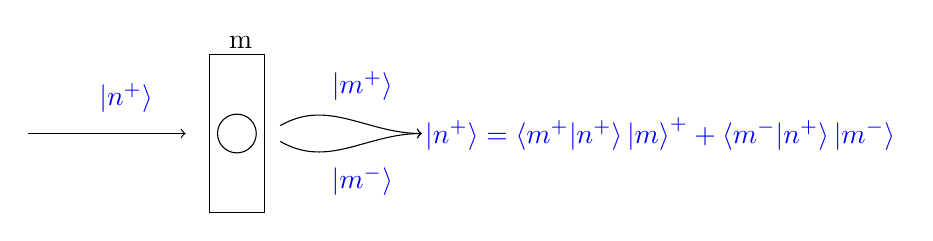
\begin{tikzpicture}
        \draw[->] (0, 0) -- (2, 0) node[yshift=3ex, xshift=-5ex, blue]{$\ket{n^+}$};
        \draw (2.3, -1) rectangle (3, 1) node[xshift=-2ex, yshift=1ex]{m};
        \draw (2.65, 0) circle (7pt);
        \draw[->] (3.2, 0.1) to [out=30, in=180]  (5, 0) node[yshift=4ex, xshift=-5ex, blue]{$\ket{m^+}$};
        \draw[->] (3.2, -0.1)  to [out=-30, in=180]  (5, 0) node[yshift=-4ex, xshift=-5ex, blue]{$\ket{m^-}$};
        \node[xshift=20ex, blue] at (5, 0) {$\ket{n^+} = \brak{m^+ | n^+} \ket m^+ + \brak{m^- | n^+}\ket{m^-}$};
    \end{tikzpicture}
\end{center}

\subsection*{Expectations}
\begin{align*}
    \E[\lambda_n |\; \ket{\Psi} = \ket{m^+}] &= |\brak{n^+ | m^+}|^2 - |\brak{n^- | m^+}|^2\\
    &= \frac{1 + m\cdot n}{2} - \frac{1 - m\cdot n}{2}\\
    &= m\cdot n\\
\end{align*}

Or 
\begin{align*}
    \E[N \ind_{\lambda_n = 1} |\; \ket{\Psi} = \ket{m^+}] &= N \cdot \E[\ind_{\lambda_n = 1} | \; \ket{\Psi} = \ket{m^+}]\\
    &= N |\brak{m^+ | n^+}|^2
\end{align*}

\section*{Lecture 9: Sept 25}
\subsection*{Mixtures and Superposition}
By now, we have 
\[\ket r = \frac{1}{\sqrt 2} \ket u + \frac{1}{\sqrt 2} \ket d\]

We want to calculate $\E[\lambda_x | \; \ket \Psi = \ket r]$

\textbf{Mixture interpretation}

We assume that because $\ket u$ and $\ket r$ are orthogonal, putting an $\ket \Psi = \ket r$ prepared vector through an $x$ machine will show it go up half the time and down half the time:
\begin{align*}
    \E[\lambda_x | \; \ket \Psi= \ket r] &= \frac{1}{2}\E[\lambda_x | \; \ket{\Psi} = \ket{u}] + \frac{1}{2}\E[\lambda_x | \; \ket{\Psi} = \ket{d}]\\
    &= \frac{1}{2}\cdot 0 + \frac{1}{2}\cdot 0\\
    &= 0
\end{align*}

But in reality, 
\[\E[\lambda_x | \; \ket \Psi = \ket r] = \P(\lambda_x = 1 | \; \ket{\Psi} = \ket{r}) - \P(\lambda_x = -1 | \; \ket{\Psi} = \ket{r}) = 1\]

\textbf{So $\ket{r}$ is NOT a mixture of $\ket{u}$ and $\ket{d}$. It is both at the same time.}

\subsection*{Measurements}
\textbf{Hermitian Adjoint:}
\[A \in \C^{m \times n}: A^\dagger= (A')^* = (A^*)'\]

\emph{Example:}
\[A = \begin{pmatrix}
    i & 2\\
    1 + i & 1 - i\\
    3 & 2i
\end{pmatrix} \implies A^\dagger = \begin{pmatrix}
    -i & 1-i & 3\\
    2 & 1+i & -2i
\end{pmatrix}\]

\textbf{Hermitian Matrix/Operator/Transform:}
\[A \in \C^{n \times n}: A^\dagger = A\]

\emph{Example:}
\[A = \begin{pmatrix}
    3 + 2i & 1-i\\
    1 - i & 2 + i
\end{pmatrix} \implies A^\dagger = \begin{pmatrix}
    3 - 2i & 1 + i\\
    1 + i & 2-i
\end{pmatrix} \implies A \neq A^\dagger \text{ so A is not Hermitian}\]

\[A = \begin{pmatrix}
    7 & 1 + i\\
    1 - i & 8
\end{pmatrix} \implies A^\dagger = A \text{ so A is Hermitian}\]

\textbf{Spectral Theorem:}

$A \in \C^{n\times n}$ is a Hermitian matrix if and only if $A$ has the form 
\[A = \sum_{k=1}^n \lambda_k e_k e_k^\dagger = \sum_{k=1}^n \lambda_k \ket{e_k}\bra{e_k}\]
where 
\begin{itemize}
    \item $\lambda_1, \;\dots, \; \lambda_n \in \R$
    \item $e_1, \; \dots, \; e_n \in \C^n$
    \item (The vectors are orthonormal:)
    \[\brak{e_k | e_l} = e_k^\dagger e_l = \delta_{kl} = \begin{cases}
        1 \quad \text{if } k = l\\
        0 \quad \text{if } k \neq l
    \end{cases}\]
\end{itemize}
(i.e. $e_1, \; \dots, \; e_n$ are orthonormal eigenvectors with eigenvalues $\lambda_1, \;\dots, \; \lambda_n$)

\section*{Lecture 10: Sept 27}
\subsection*{Examples of the Spectral Theorem}
\textbf{Example 1:}
\[H = \begin{pmatrix}
    3 & -i\\
    i & 3
\end{pmatrix}\]

By the Spectral Theorem,
\begin{align*}
    H &= \lambda_1 e_1 e_1^\dagger + \lambda_2 e_2 e_2^\dagger\\
    &= 2\begin{pmatrix}
        \frac{1 + i}{2}\\
        \frac{1 - i}{2}
    \end{pmatrix}\begin{pmatrix}
        \frac{1 + i}{2}\\
        \frac{1 - i}{2}
    \end{pmatrix}^\dagger + 4\begin{pmatrix}
        \frac{1 + i}{2}\\
        \frac{-1 + i}{2}
    \end{pmatrix}\begin{pmatrix}
        \frac{1 + i}{2}\\
        \frac{-1 + i}{2}
    \end{pmatrix}^\dagger
\end{align*}

How do we check this? 

Answer:
\[He_1 = 2e_1 \quad He_2 = 4e_2\]
(the action of the matrix on two orthogonal vectors defines the matrix)

\subsection*{Proof of the Spectral Theorem}
\textbf{Lemma:} For a Hermitian matrix,
\[H = \sum_{k=1}^n \lambda_k e_k e_k^\dagger,\]
the values $\lambda_k \in \R$.

\emph{Proof:}

Let $\lambda$ be an eigenvalue with eigenvector $e$. Then 
\begin{align*}
    \lambda &= e^\dagger He\\
    \lambda^* = \lambda^\dagger &= (e^\dagger He)^\dagger\\
    &= e^\dagger H^\dagger e\\
    &+ e^\dagger He\\
    &= \lambda
\end{align*}
so $\lambda$ is real. 

\textbf{Remark:} the collection of eigenvalues $\lambda_k$ are called the ``spectrum''

\section*{Lecture 11: Sept 29}
\subsection*{Motivating Hermitian Operators}
Needing matrices becomes natural when we view state space as hilbert space and the matrices as linear operators on hilbert space. 

\textbf{Goal:} find an operator $o$ that maps a wave function to a particular state. 

One potential is $\ket \Psi \to \ket{n^+}$ using the \textbf{projection operators:}
\[\ket{n^+}\bra{n^+}, \qquad \ket{n^-}\bra{n^-}\]

If we imagine $\sigma_n$ as a particular state, then 
\begin{align*}
    \sigma_n\ket{n^+} &= \frac{\hbar}{2}\ket{n^+}\\
    \sigma_n \ket{n^-} &= -\frac{\hbar}{2}\ket{n^-}
\end{align*}
So we note that there is a distinction between states ($\in \C_1^2$) and values (in $\R$)

Actually working it out, 
\begin{align*}
    \sigma_n := \ket{n^+}\bra{n^+} - \ket{n^-}\bra{n^-}\\
    \sigma_s \ket{n^+} &= \ket{n^+} \brak{n^+ \; | \; n^+} - \ket{n^-}\brak{n^- \; | \; n^+}\\
    &= \ket{n^+} (1) - \ket{n^-}(0) = \ket{n^+}
\end{align*}

\subsection*{Observables}
\textbf{Definition:} a Hermitian operator $\sum_i \lambda_i \ket{e_i} \bra{e_i}$ with eigenvectors corresponding to states after measurement $\ket{e_i}$ and eigenvalues $\lambda_i$ corresponding to the physical values we measure ($\{\pm \frac{\hbar}{2}\} \mapsto \{\pm 1\}$). 

This also suggests that $\big\vert \brak{e_i \; | \; \Psi}
\big\vert^2$ is the probability of collapse onto a particular state $\ket{e_i}$ 

\subsection*{Computing spin states}
\begin{align*}
    \sigma_z &= \ket{z^+} \bra{z^+} - \ket{z^-}\bra{z^+}\\
    &+ \begin{pmatrix}
        1 & 0
    \end{pmatrix}\begin{pmatrix}
        1\\0 
    \end{pmatrix} - \begin{pmatrix}
        0 & 1
    \end{pmatrix} \begin{pmatrix}
        0\\1
    \end{pmatrix}\\
    &= \begin{pmatrix}
        1 & 0\\
        0 & 0
    \end{pmatrix} - \begin{pmatrix}
        0 & 0\\
        0 & 1
    \end{pmatrix}\\
    &= \begin{pmatrix}
        1 & 0\\
        0 & -1
    \end{pmatrix}
\end{align*}
Which we notice is a diagonal matrix with eigenvalues $\pm 1$. 

In the same process, 
\begin{align*}
    \ket{x^\pm} &= \frac{1}{\sqrt 2}(\ket{z^+} \pm \ket{z^-})\\
    \ket{y^\pm} &= \frac{1}{\sqrt 2}(\ket{z^+} \pm i\ket{z^-})\\
    \sigma_x &= \ket{x^+} \bra{x^+} - \ket{x^-}\bra{x^+} = \begin{pmatrix}
        0 & 1\\
        1 & 0
    \end{pmatrix}\\
    \sigma_y &= \begin{pmatrix}
        0 & -i\\
        i & 0
    \end{pmatrix}
\end{align*}

However, these matrices tell us nothing about the states or eigenvalues. To take any probabilities $\big\vert\brak{z^+ \; | \; x^+}\big\vert^2$ we would need to know the explicit form of both vectors. But! We can \emph{diagonalize} a given matrix to find the probability for any matrix. 

Taken together, these three basis matrices are the \emph{Pauli Matrices:}
\begin{empheq}[box=\fbox]{align*}
    \sigma_z &= \begin{pmatrix}
        1 & 0\\
        0 & -1
    \end{pmatrix}\\
    \sigma_x &= \begin{pmatrix}
        0 & -i\\
        i & 0
    \end{pmatrix}\\
    \sigma_y &= \begin{pmatrix}
        0 & -i\\
        i & 0
    \end{pmatrix}    
\end{empheq}

\subsection*{Expected Value}
\[A = \sum_i \lambda_i \ket{e_i} \bra{e_i}\]F
From probability theory, the expected value is just the sum of the probability times the value: 
\begin{align*}
    \E(A \; | \; \ket{\Psi}) &= \sum_i \big\vert \brak{e_i \; | \; \Psi} \big \vert^2 \lambda_i\\
    & = \sum_i \brak{\Psi \; | \; e_i} \brak{e_i \; | \; \Psi} \lambda_i\\
    &= \brak{\Psi}\left(\sum_i \ket{e_i} \bra{e_i} \lambda\right)\ket{\Psi}\\
    &= \brak{\Psi \; | \; A \; | \;\Psi}
\end{align*}

\section*{Lecture 12: Oct 2}
\subsection*{Recall}
We can represent a particular observation by the Hermitian matrix $H$:
\[H = \sum_{k=1}^n \lambda_k \ket{e_k} \bra{e_k}\]
where the vectors $e_k$ form a complete orthonormal set and $\lambda_k \in \R$. 

Then, given the starting state $\ket{\Psi}$, the probability of the random result of making the observation represented by $H$, is 
\[\P(\lambda_H = \lambda_k \; | \; \ket{\Psi}) = \big\vert \brak{e_k \; | \; \Psi}\big \vert^2\]

This leads to the formula for expected value:
\begin{align*}
    \E[\lambda_H \; | \; \ket \Psi] &= \sum_{k=1}^n \lambda_k \P(\ket{e_k})\\
    &= \sum_{k=1}^n \big\vert \brak{e_k \; | \; \Psi} \big\vert^2\\
    &= \brak{\Psi \; | \; H \; | \; \Psi}
\end{align*}

\subsection*{Multiple measurements}
\textbf{Example:} $H_1 = \sigma_x$ and $H_2 = -\sigma_x$ with $\ket \Psi = \ket r$. Then $\lambda_1 = 1$ and $\lambda_2 = -1$ (deterministically).

In general, if $H_1$ and $H_2$ share eigenvectors, then order is ``independent'':
\[\ket \Psi \overunderset{H_1}{\lambda_k^1}{\longrightarrow} \ket{e_k^1} \overunderset{H_2}{\lambda_l^2}{\longrightarrow} \ket{e_l^2}\]

\textbf{Question:} When is $A = H_2 \cdot H_1$ a measurement? (i.e. when is it Hermitian?)

\emph{Answer:} If and only if $H_1$ and $H_2$ are both hermitian and share the same eigenvectors:
\begin{align*}
    H_1 &= \sum_{k=1}^n \lambda_k^1 \ket{e_k} \bra{e_k}\\
    H_2 &= \sum_{k=1}^n \lambda_k^2 \ket{e_k} \bra{e_k}
\end{align*}
(the eigenvalues can be different but the eigenvectors are the same)

\textbf{Definition:} The \emph{commutator} of $AB$ is 
\[[AB] = AB - BA\]
so $A$ and $B$ commute iff $[AB] = 0$

\section*{Lecture 13: Oct 6}

\section*{Lecture 14: Oct 11}
\textbf{The Schrodinger Equation:} Moves state forward in time deterministically based on state, environment, and time 

\subsection*{Setup}
We want a transformation $U$ that maps 
\[\begin{pmatrix}
    0\\1
\end{pmatrix} \to \begin{pmatrix}
    1\\0
\end{pmatrix} \quad \text{and} \quad \begin{pmatrix}
    1\\0
\end{pmatrix}\to \begin{pmatrix}
    0\\1
\end{pmatrix}\]

Two options are 
\begin{align*}
    \begin{pmatrix}
        0 & 1\\ 
        1 & 0
    \end{pmatrix}\begin{pmatrix}
        0\\1
    \end{pmatrix} &= \begin{pmatrix}
        1\\0
    \end{pmatrix}\\
    \begin{pmatrix}
        0 & 1\\ 
        -1 & 0
    \end{pmatrix}\begin{pmatrix}
        1\\0
    \end{pmatrix} &=   
    \begin{pmatrix}
        0\\-1
    \end{pmatrix} 
\end{align*}
Notice the second resultant is in the equivalence class of $\ket d$ with respect to phase. 

\textbf{Notation:} $\ket{\Psi(t)} = U_t\ket{\Psi(0)}$

\subsection*{Derivation}
\textbf{Desiderata:}
\begin{enumerate}
    \item Linearity:
    \[U_t (\ket{\Psi_1(0)} + \ket{\Psi_2(0)}) = U_t\ket{\Psi_1(0)} + U_t\ket{\Psi_2(0)} = \ket{\Psi_1(t)} + \ket{\Psi_2(t)}\]

    \item Conservation of Probability (i.e. $\ket{\Psi(t)} \in \C_1^2$)
    \[\brak{\Psi(t) \; | \; \Psi(t)} = 1 \quad \forall t\]
\end{enumerate}
Already from these properties, we have a vector space and linearity so $U_t$ has a matrix representation: $U_t \in \C^{2 \times 2}$. 

Then from the second condition, be substitution,
\begin{gather*}
    \ket{\Psi(t)} = U_t\ket{\Psi(0)}\\ 
    \brak{\Psi(t) \; | \; \Psi(t)} = 1\\ 
    (U_t \ket{\Psi(0)})^\dagger (U_t \ket{\Psi(0)}) = 1\\
    \brak{\Psi(0) U_t^\dagger U_t \; | \; \Psi(0)} = 1\\
\end{gather*}
But since $(U^\dagger U)^\dagger = U^\dagger U$, we know $U^\dagger U$ is Hermitian. So we can write 
\[U_t^\dagger U_t = \sum_{i=1}^n \lambda_k \ket{e_k}\bra{e_k}\]

Plugging back in,
\begin{align*}
    \brak{\Psi \bigg\vert \sum_{i=1}^n \lambda_k \ket{e_k}\bra{e_k} \bigg\vert \Psi} = 1 \quad \forall \Psi
\end{align*}
But as this is true \emph{for all} states, we can arbitrarily choose $\Psi = e_l$ so 
\[\brak{e_l \bigg\vert \sum_{i=1}^n \lambda_k \ket{e_k}\bra{e_k} \bigg\vert e_l} = \lambda_l = 1\]

Hence, all the eigenvalues are 1. Further, $U^\dagger U = I$

\textbf{Unitary:} a matrix $U: \C_1^n \to \C_1^n$ such that 
\[U^\dagger U = UU^\dagger = I\]

All together, 
\[\brak{\Psi(0) \; | \; U_t^\dagger U_t \; | \; \Psi(0)} = \brak{\Psi(0) \; | \; I \; | \; \Psi(0)} = \brak{\Psi(0) \; | \; \Psi(0)} = \brak{\Psi(t) \; | \; \Psi(t)}\]

More generally, 
\[\brak{\Psi_1(0) \; | \; \Psi_2(0)} = \brak{\Psi_1(0) \; | \; U_t^\dagger U \; | \; \; | \Psi_2(0)} = \brak{\Psi_1(t) \; | \; \Psi_2(t)}\]
So $U_t$ preserves overlap. 

\section*{Lecture 15: Oct 13}
\subsection*{Unitary Matrices}
\textbf{Definition:} if a matrix $U: \C_1^n \to \C_1^n$ and 
\[U^\dagger U = UU^\dagger = 1\]

\textbf{Examples:}
\begin{itemize}
    \item $R_\theta = \begin{pmatrix}
        \cos \theta & -\sin \theta\\
        \sin \theta & \cos \theta
    \end{pmatrix}$ is unitary but not Hermitian

    \item $\sigma_y = \begin{pmatrix}
        0 & -i\\
        i & 0
    \end{pmatrix}$ is unitary and Hermitian 
\end{itemize}

\subsection*{Schrodinger Derivation (Continued)}
\textbf{Recall:} by demanding linearity and conservation of probability we have shows that for any starting states,
\[\brak{\Psi_1(0) \; | \; \Psi_2(0)} = \brak{\Psi_1(0) \; | \; U_t^\dagger U \; | \; \; | \Psi_2(0)} = \brak{\Psi_1(t) \; | \; \Psi_2(t)}\]

Now we introduce another condition:
\begin{enumerate}
    \setcounter{enumi}{2}
    \item State: 
    \[U_{t + s} = U_t U_s\]
    so 
    \[\ket{\Psi(t + s)} = U_{t + s} \ket{\Psi(0)} = U_t \ket{\Psi(s)}\]

    \item Continuity: 
    \[\lim_{s \to 0} U_{t+s} \ket \phi = U_t \ket \phi\]
    Concretely,
    \[\lim_{s\to 0} \ket{\Psi(t + s)} = \ket{\Psi(t)}\]
\end{enumerate}

\textbf{Stone's Representation Theorem:} If $U_{t\geq 0}$ satisfies linearity, unitarity, and continuity then there exists a Hermitian operator $A: \C^n \to \C^n$ such that 
\[U_t = e^{iAt}\]

\textbf{Interlude: Functions of Hermitian Operators}

Recall that if $A$ is Hermitian, then 
\[A = \sum_{k=0}^n \lambda_k \ket{e_k}\bra{e_k}\]
and 
\[A^2 = \sum_{k} \sum_{l} \lambda_k \lambda_l \ket{e_k} \brak{e_k \; | \; e_l}\bra{e_l} = \sum_{k=0}^n \lambda_k^2 \ket{e_k}\bra{e_k}\]

If we let $f(x) = x^2$ then 
\[f(A) = \sum_{k=0}^n f(\lambda_k) \ket{e_k}\bra{e_k}\]

From analysis you can generalize to all powers, then all polynomials (by linearity), then eventually continuity. 

\textbf{Back to Stone's:}

In particular, if $f(x) = e^{itx}$ then 
\[f(A) = e^{itA}\]
so by Stone's theorem
\[\ket{\Psi(t)} = U_t\ket{\Psi(0)} = e^{itA}\ket{\Psi(0)}\]

Now taking the derivative, we get Schrodinger's Equation:
\[\boxed{\frac{d}{dt}\ket{\Psi(t)} = iAe^{itA}\ket{\Psi(0)} = iA\ket{\Psi(t)}}\]

Now applying the state definition,
\[\ket{\Psi(t)} = \begin{pmatrix}
    \alpha(t)\\
    \beta(t)
\end{pmatrix} \in \C^2\]
and 
\[A = \begin{pmatrix}
    a_{11} & a_{12}\\
    a_{21} & a_{22}
\end{pmatrix}\]
so 
\[\begin{cases}
    \dot \alpha = ia_{11}\, \alpha(t) + ia_{21}\,\beta(t)\\
    \dot \beta = ia_{21}\, \alpha(t) + ia_{22}\,\beta(t)
\end{cases}\]

\section*{Lecture 16: Oct 16}
\subsection*{Tensor Product Space}
\textbf{Notation:} with $V = \C^n$ and $W = \C^m$, two vector spaces containing a particle in each. We let $V \otimes W$ is the state space of pairs of particles $V$ and $W$. We make the natural assumptions:
\begin{enumerate}
    \item $V \otimes W$ is a complex vector space 
    \item It has an inner product ($\ket \Psi, \ket \Phi \in V\otimes W \implies \brak{\Psi \; | \; \Phi} \in \C$) which is linear in $\ket \Phi$ and conjugate-linear in $\ket \Psi$
\end{enumerate}

\textbf{Construction (Ansatz):}
\begin{enumerate}
    \item (Assumption) Minimal elements: $\forall \ket v \in V,\; \ket w \in W$ assume that the independent pair (designated $\ket{v\;w}$) is in $V \otimes W$. 
    
    \item Overlap: with $\ket \Psi, \ket \Phi \in V\otimes W$, 
    \[\P(\ket \Psi \overset{A}{\to} \ket \Phi) = \bigg\vert \brak{\Psi \; | \; \Phi}_{V \otimes W} \bigg\vert^2\]

    \item Independence: if we have two experiments $\ket v \overset{A}{\to} \ket{\tilde{v}}$ and $\ket w \overset{B}{\to} \ket{\tilde w}$ with the pair in A being independent from the pair in $B$, then 
        \begin{align*}
            \bigg\vert \brak{v w \; | \; \tilde v \tilde w}_{V \otimes W} \bigg\vert^2 &= \P(\ket{vw} \to \ket{\tilde v \tilde w})\\
            &= \P([\ket{v} \overset{A}{\to} \ket{\tilde v}] \cap [\ket{w} \overset{B}{\to} \ket{\tilde w}])\\
            &= \P(\ket{v} \overset{A}{\to} \ket{\tilde v}) \cdot \P(\ket{w} \overset{B}{\to} \ket{\tilde w})\\
            &= \Big\vert \brak{v \; | \; \tilde v}_{V} \Big\vert^2 \;\; \Big\vert \brak{w \; | \; \tilde w}_{W} \Big\vert^2
        \end{align*}

        \item Existence of $nm$ orthonormal states in $V \otimes W$:
            Let $\ket{e_1}, \dots, \, \ket{e_n} \in V$ and $\ket{f_1}, \dots,\, \ket{f_n} \in W$ be orthonormal sets. Then $\forall 1 \leq i \leq n, 1 \leq j \leq m$ $\ket{e_i f_j} \in V \otimes W$ and 
            \[\brak{e_i f_j \; | \; e_k f_l}_{V \otimes W} = \brak{e_i \; | \; e_k}_V \otimes \brak{f_j \; | \; f_l}_W = \delta_{ik} \delta_jl\]
            so $\{\ket{e_i f_j}\}$ is an orthonormal set in $V \otimes W$. This immediately tells us that all linear combinations of these vectors is in the space:
            \[\left\{\sum_{i=0}^n \sum_{j=0}^m \gamma_{ij} \ket{e_i f_j} \bigg\vert \gamma_{ij} \in \C\right\} \subseteq V \otimes W\]
            Is this enough to form a full basis for the space? 

        \item Occam's Razor: We assume that the basis described above \emph{is} sufficient to form a basis for $V \otimes W$
\end{enumerate}

\section*{Lecture 17: Oct 18}
\subsection*{Review of the Tensor Space}
We have two particles $w \in W$ and $v \in V$ where $V \in \C^n$ and $W \in \C^m$ are state spaces. 

We define $V \otimes W$ as a vector inner-product space such that 
\begin{enumerate}
    \item $\forall \ket \Psi, \ket \Phi \in V \otimes W, \quad \brak{\Psi \; | \; \Phi} \in \C$
    \item We assume that $V \otimes W$ contains an element for all pair of states $\ket v \in V$, $\ket w \in W$ which we designate as 
    \[\ket{vw} = \ket v \otimes \ket w \in V\otimes W\]
    \item \[\brak{vw \; | \; \tilde v \tilde w}_{V \otimes W} = \brak{v \; | \; \tilde v}\brak{w \; | \; \tilde w}\]
    \item Given orthonormal basis sets $\{\ket{e_1}, \dots,\, \ket{e_n}\}$ for $V$ and $\{\ket{f_1}, \dots,\, \ket{f_m}\}$ for $W$, 
    \[V \otimes W = \left\{\sum_{i=1}^n \sum_{j=1}^m \gamma{ij} \ket{e_i f_j} \; | \;\gamma_{ij} \in \C\right\}\]
    \item If $\ket \Psi = \sum_{i, j} \alpha_{ij} \ket{e_i f_j}$ and $\ket{\Phi} = \sum_{k,l} \beta_{kl} \ket{e_k f_l}$, then  
    \[\brak{\Psi \; | \; \Phi} = \sum_{ij} \alpha^*_{ij} \beta_{ij}\]
\end{enumerate}

\textbf{Remarks:} 
\begin{itemize}
    \item $\{\ket{e_i f_j} \; | \; 1 \leq i \leq n, 1 \leq j \leq m\}$ is orthonormal of size $mn$ so it is a basis. 
    \item Construction is independent of basis (because of linear algebra and the inner product)
    \item Condition 4 is actually redundant and arises naturally from the inner product
\end{itemize}

\textbf{Independence:} If $\ket \Psi = \ket{vw} = \ket v \otimes \ket w$ for some $\ket v \in V$, $\ket w \in W$ then $v$ and $w$ are \emph{independent}. Otherwise, they are \emph{entangled}.

Now we might wonder if we can go the other way: When is $\ket \Psi = \sum_{ij} \gamma_{ij} \ket{e_i f_j}$ the state of a pair of independent particles? 

\textbf{Theorem:} $\ket \Psi$ consists of two independent states if and only if 
\[\exists a_1, \dots,\, a_n \in C, b_1, \dots,\, b_m \in C\]
such that $\gamma_{ij} = a_i b_j$

This leads to another property: If $\sum a_i \ket{e_i} \in \C_1^n$ and $\sum b_j \ket{f_j} \in \C_1^m$, then  
    \[\sum_{i=1}^n \sum_{j=1}^m \big\vert a_i b_j \big\vert^2 = 1\] 
    or 
    \[\sum_{ij} a_ib_k \ket{e_i f_j} \in \C_1^{n\times m} = \C^n \otimes \C^m\]

\subsection*{Example: the ``singlet state''}
In $\C^2 \otimes \C^2$, if we have one particle 
\[\ket \Psi = \frac{1}{\sqrt 2} \ket{ud} - \frac{1}{\sqrt 2}\ket{du}\]
and we measure one of the two, then we immediately know the state of the other

\end{document} 
